\documentclass{beamer}
\usepackage{graphicx}
\usepackage{tikz}
\usetikzlibrary{shapes,arrows}
\usepackage{tikz}
\usetheme{default}
%\usecolortheme{seahorse}
\usepackage{default}

  \setbeamertemplate{footline}[page number]
\setbeamertemplate{navigation symbols}{}
\setbeamertemplate{frametitle}[default][center]
\setbeamerfont{frametitle}{shape=\scshape}

\usepackage{color}

\usepackage{media9}%
\newcommand{\includemovie}[3]{%
\includemedia[%
width=#1,height=#2,%
activate=pagevisible,%
deactivate=pageclose,%
addresource=#3,%
flashvars={%
src=#3 % same path as in addresource!
&autoPlay=true % default: false; if =true, automatically starts playback after activation (see option ?activation)?
&loop=true % if loop=true, media is played in a loop
&controlBarAutoHideTimeout=0 %  time span before auto-hide
}%
]{}{StrobeMediaPlayback.swf}}%


{\title{\textsc{Numerical Methods-Lecture IX: Quadrature (and Markov Chains)} \\ \ \\ \tiny (See Judd Chapter 7, Stokey Lucas Prescott Chapter 11)}
\author{Trevor Gallen}
\date{}

\begin{document}

\begin{frame}
\titlepage
\end{frame}

\begin{frame}
\frametitle[alignment=center]{Motivation}
\begin{itemize}
\item $E(x)=\int_{-\infty}^\infty xf(x)$ for $x$ with PDF $f(x)$
\bigskip
\item Most Bellman Problems look something like:
\bigskip
$$V(x)=\underset{y}{\max}\left\{\phi(x,y)+\beta E(V(x))\right\}$$
\bigskip
\item One option is to force our probability space to be easy to use
\bigskip
\item Another is to integrate properly (at least, within some tolerance)
\end{itemize}
\end{frame}


\begin{frame}
\frametitle[alignment=center]{Easy to use probability spaces}
\begin{itemize}
\item Markov chains are wonderfully simple
\bigskip
\item Chapter 11 of RMED
\bigskip
\item Allow your states to evolve stochastically, within bounds
\bigskip
\item Summarize probability of transition as a matrix
\end{itemize}
\end{frame}

\begin{frame}
\frametitle[alignment=center]{Markov Chains}
\begin{itemize}
\item We have some state (income, say) that consists of a finite number of elements:
\bigskip
$$S=\{s_1,s_2,...,s_n\}$$
\bigskip
\item We define the probability of transitioning from state $i$ to state $j$ by probability $\pi_{ij}$ in row $i$, column $j$:
\bigskip
$$\Pi=\left[\begin{array}{cccc}\pi_{1\rightarrow1} & \pi_{1\rightarrow2} & \cdots & \pi_{1\rightarrow n} \\ 
\pi_{2\rightarrow1} & \pi_{2\rightarrow2} & \cdots & \pi_{2\rightarrow n} \\
\vdots & \vdots & \ddots & \vdots \\
\pi_{n\rightarrow1} & \pi_{n\rightarrow2} & \cdots & \pi_{n\rightarrow n} 
 \end{array}\right]$$
\end{itemize}
\end{frame}

\begin{frame}
\frametitle[alignment=center]{Properties of Markov Chains}
$$\Pi=\left[\begin{array}{cccc}\pi_{1\rightarrow1} & \pi_{1\rightarrow2} & \cdots & \pi_{1\rightarrow n} \\ 
\pi_{2\rightarrow1} & \pi_{2\rightarrow2} & \cdots & \pi_{2\rightarrow n} \\
\vdots & \vdots & \ddots & \vdots \\
\pi_{n\rightarrow1} & \pi_{n\rightarrow2} & \cdots & \pi_{n\rightarrow n} 
 \end{array}\right]$$
\begin{itemize}
\item All rows must add up to 1!
\item If your position is summarized by row vector $V$, then the probability you'll be in each state next period is given by:
$$V_{t+1}=V_t\Pi $$
\item This is true for multiple iterations of $\pi$:
$$V_{t+1}=V_t\Pi^2 $$
\item It's easy to find the invariant distribution (if it exists) as:
$$\underset{n\rightarrow \infty}{\lim}V_t\Pi^n$$
\end{itemize}
\end{frame}

\begin{frame}
\frametitle[alignment=center]{Markov Chain: Death Example}
$$\Pi=\left[\begin{array}{ccccccccc}
0 & 0.9 & 0 & 0 & 0 & 0 & 0 & 0 & 0.1 \\
0 & 0 & 0.8 & 0 & 0 & 0 & 0 & 0 & 0.2 \\
0 & 0 & 0 & 0.7 & 0 & 0 & 0 & 0 & 0.7 \\
0 & 0 & 0 & 0 & 0.96 & 0 & 0 & 0 & 0.04 \\
0 & 0 & 0 & 0 & 0 & 0.6 & 0 & 0 & 0.6 \\
0 & 0 & 0 & 0 & 0 & 0 & 0.7 & 0 & 0.7 \\
0 & 0 & 0 & 0 & 0 & 0 & 0 & 0.8 & 0.2 \\
0 & 0 & 0 & 0 & 0 & 0 & 0 & 0.7 & 0.3\\
0 & 0 & 0 & 0 & 0 & 0 & 0 & 0 & 1
\end{array}\right]$$
\begin{itemize}
\item Where I interpret entries as $\{a_1,a_2,a_3,a_4,a_5,a_6,a_7,a_8,Death\}$
\item Interpret 
\end{itemize}
\end{frame}

\begin{frame}
\frametitle[alignment=center]{Markov Chain: Death Example}
\begin{itemize}
\item Starting at $$V_0=[1,0,0,0,0,0,0,0,0,0]$$
Apply $\Pi$ repeatedly:
 $$V_1=  [\begin{array}{ccccccccc}1  &  0  &  0  &  0  &  0  &  0  &  0  &  0  &  0 \end{array}]$$
 $$V_2=  [ \begin{array}{ccccccccc}  0 &    0.9  &  0  &  0  &  0  &  0  &  0  &  0 &    0.1\end{array}]$$
 $$V_3=  [\begin{array}{ccccccccc}  0  &  0 &   0.63  &  0  &  0  &  0  &  0  &  0 &   0.37\end{array}]$$
   $$V_4=[\begin{array}{ccccccccc}    0  &  0  &  0 &  0.57  &  0  &  0  &  0  &  0 &  0.43\end{array}]$$
   $$V_5=[\begin{array}{ccccccccc}    0  &  0  &  0  &  0 & 0.56  &  0  &  0  &  0 & 0.44\end{array}]$$
   $$V_6=[\begin{array}{ccccccccc}    0  &  0  &  0  &  0  &  0   &   0.39  &  0  &  0 & 0.61\end{array}]$$
   $$V_7=[\begin{array}{ccccccccc}    0  &  0  &  0  &  0  &  0  &  0   &   0.24  &  0 & 0.76\end{array}]$$
   $$V_8=[ \begin{array}{ccccccccc}   0  &  0  &  0  &  0  &  0  &  0  &  0 & 0.12 & 0.88\end{array}]$$
   $$V_9= [\begin{array}{ccccccccc}   0  &  0  &  0  &  0  &  0  &  0  &  0 & 0.05 & 0.95\end{array}]$$
   $$V_{10}=[ \begin{array}{ccccccccc}   0  &  0  &  0  &  0  &  0  &  0  &  0 & 0.02 & 0.98\end{array}]$$
   $$V_{11}=[ \begin{array}{ccccccccc}   0  &  0  &  0  &  0  &  0  &  0  &  0 & 0.01 & 0.99\end{array}]$$
\end{itemize}
\end{frame}

\begin{frame}
\frametitle[alignment=center]{Markov Chain: Death Example}
\begin{figure}
\centering
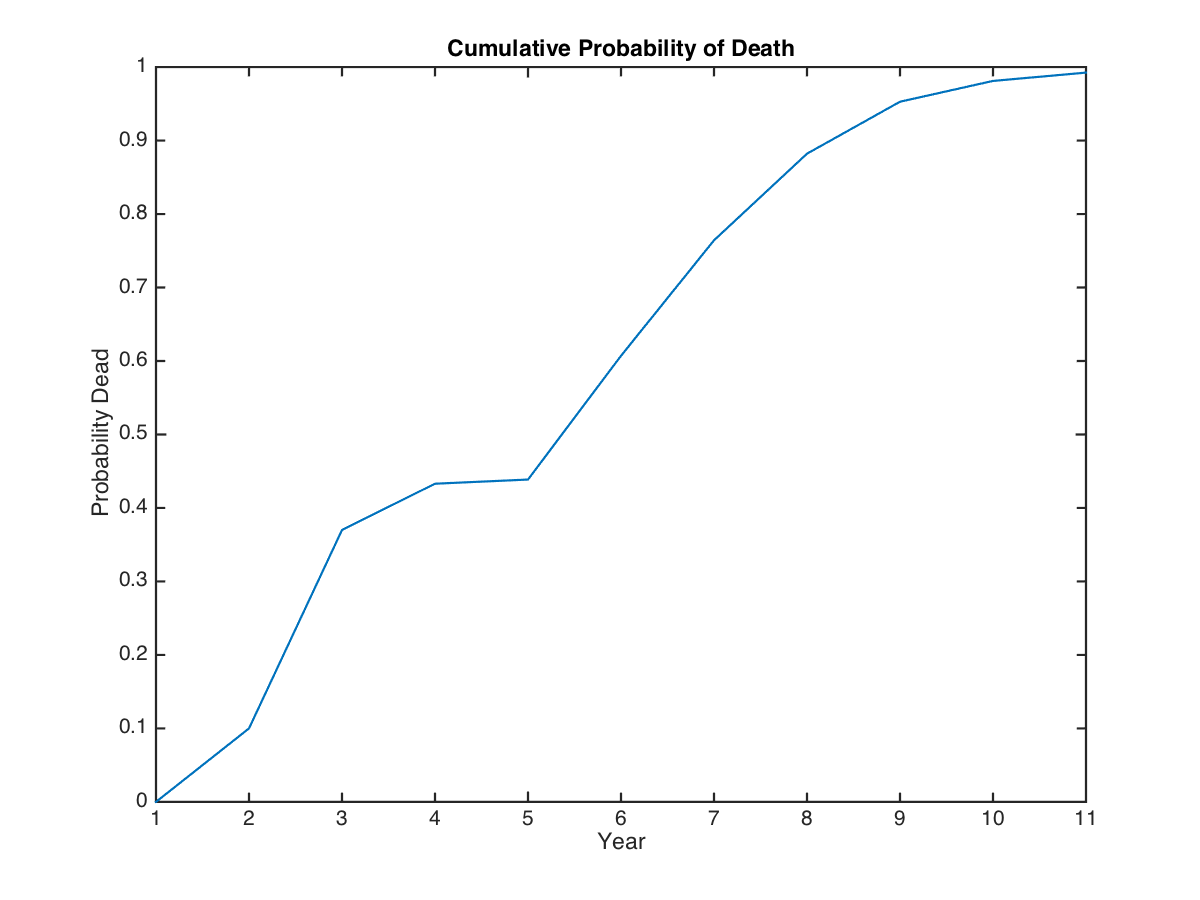
\includegraphics[scale=0.5]{CumulativeProbDeath.png}
\end{figure}
\end{frame}

\begin{frame}
\frametitle[alignment=center]{Regime Shifts}
\begin{itemize}
\item We could also model persistent``regime shifts"
$$\Pi=\left[\begin{array}{cc}0.99 & 0.01 \\ 0.01 & 0.99\end{array}\right]$$
\end{itemize}
\begin{figure}
\centering
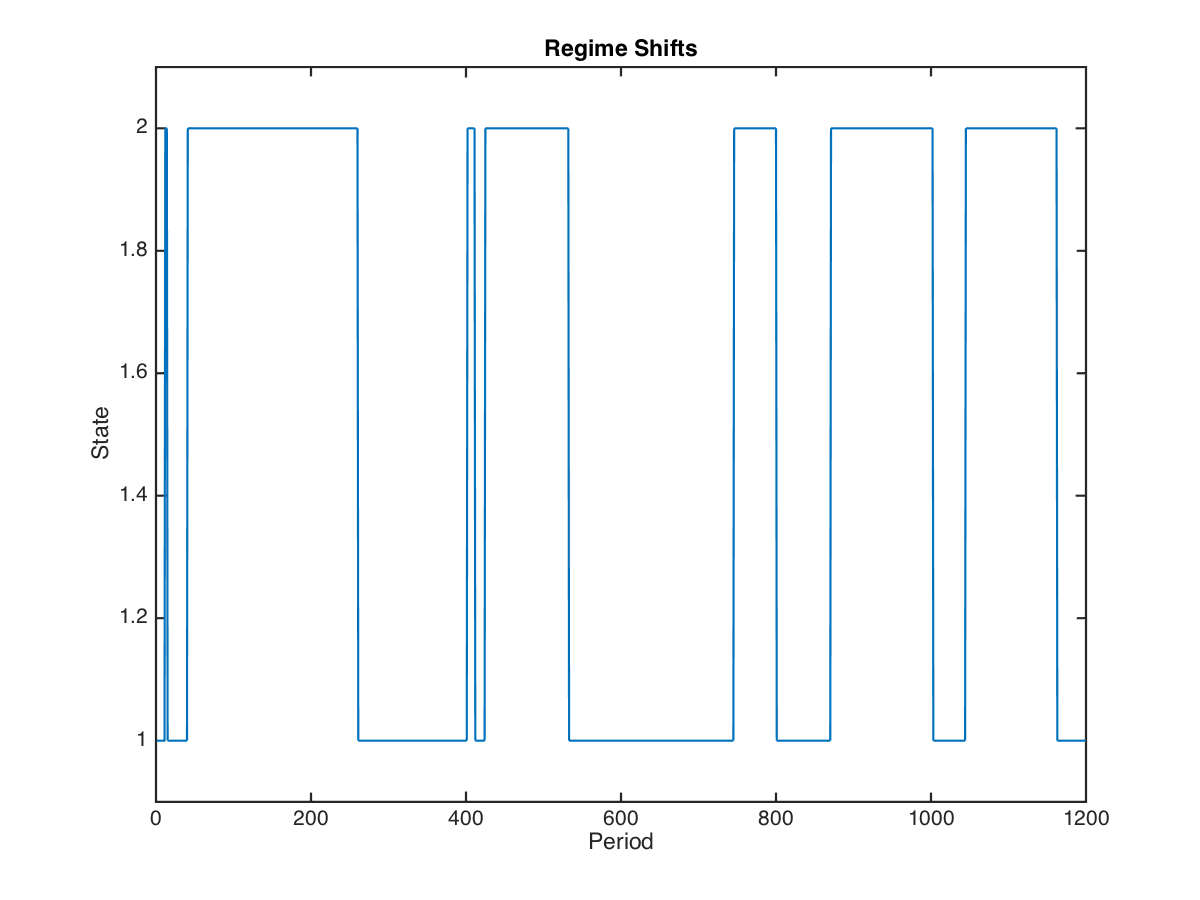
\includegraphics[scale=0.4]{RegimeShifts.png}
\end{figure}
\end{frame}

\begin{frame}
\frametitle[alignment=center]{Sudden Brief Shocks}
\begin{itemize}
\item We could also model sudden and brief shocks
$$\Pi=\left[\begin{array}{cc}0.99 & 0.01 \\ 0.3 & 0.7\end{array}\right]$$
\end{itemize}
\begin{figure}
\centering
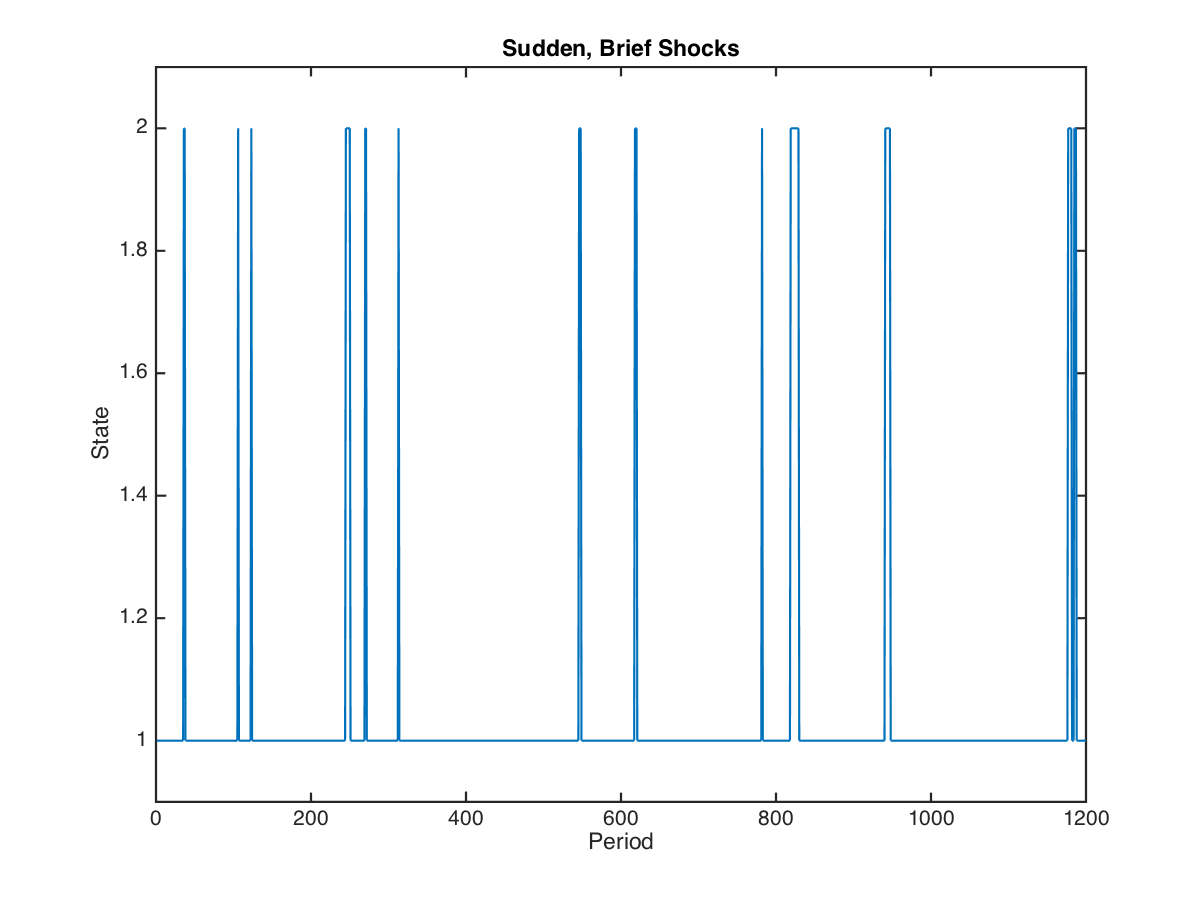
\includegraphics[scale=0.4]{SuddenShocks}
\end{figure}
\end{frame}

\begin{frame}
\frametitle[alignment=center]{Period of Uncertainty}
\begin{itemize}
\item We could model a ``time of uncertainty"
$$\Pi=\left[\begin{array}{ccc}0.99 & 0.01 & 0 \\ 0.5 & 0 & 0.5 \\ 0 & 0.01 & 0.99\end{array}\right]$$
\item You could imagine a model of investment under uncertainty
\item When in state 1 or 3, you know the deal
\item If in state 2, wait to find out what state you're in next period
\end{itemize}
\end{frame}

\begin{frame}
\frametitle[alignment=center]{Cyclical Behavior}
\begin{itemize}
\item Some stochastic behavior is cyclical
$$\Pi=\left[\begin{array}{ccccc}0.5 & 0.5 & 0 & 0 & 0\\ 0 & 0.5 & 0.5 & 0 & 0 \\ 0 & 0 & 0.5 & 0.5 & 0 \\ 0 & 0 & 0 & 0.5 & 0.5 \\ 0.5 & 0 & 0 & 0 & 0.5\end{array}\right]$$
\item The real minimum wage doesn't look dissimilar to this (if you assign states properly)
\end{itemize}
\end{frame}


\begin{frame}
\frametitle[alignment=center]{Markov Chains: Summary}
\begin{itemize}
\item Very flexible, incredibly easy to use, program, simulate
\bigskip
\item Easy to estimate using maximum likelihood
\bigskip
\item Good for learning problems or any regime shifting problems
\bigskip
\item Require discrete states
\bigskip
\item Easy to ``integrate" and get probabilities
\bigskip
\item Don't leave home without them
\end{itemize}
\end{frame}

\begin{frame}
\frametitle[alignment=center]{Quadrature}
\begin{itemize}
\item Frequently, one wants to use continuous probability distributions 
\bigskip
\item It turns out there are a bunch of rules that get us very accurate integrals from a finite sampling of points
\bigskip
\item Theoretically, you all basically learned one method $\sim$ 5 years ago...
\end{itemize}
\end{frame}

\begin{frame}
\frametitle[alignment=center]{Quadrature: Basic Idea}
\begin{itemize}
\item Let's say we want to integrate $\sin(x)$ over a uniform distribution from $(0,2\pi)$
\bigskip
\item Take 3 points: $\frac{\pi}{3}$, $\pi$, and $\frac{5}{3}\pi$, assign the surrounding $\frac{\pi}{3}$ on both sides to them.
\end{itemize}
\end{frame}

\foreach \x in {1,...,9}{
\begin{frame}
\frametitle[alignment=center]{Quadrature: Basic Idea}
\begin{figure}
\centering
\includegraphics[scale=0.5]{Riemann_\x.png}
\end{figure}
\end{frame}
}

\begin{frame}
\frametitle[alignment=center]{We can do better}
\begin{itemize}
\item Two choices: where points are, and weights of points
\bigskip
\item We chose equal weights, equidistant points
\bigskip
\item Simpson's rule takes better weights:
\bigskip
$$\int_a^bf(x)dx\approx \frac{b-a}{6}\left(f(a)+4f\left(\frac{a+b}{2}\right)+f(b)\right)$$
\bigskip
\item Break up into six points, heavily weight the middle
\bigskip
\item This results from a quadratic approximation
\bigskip
\item Simpson's rule is a special case of Newton-Coates
\end{itemize}
\end{frame}


\begin{frame}
\frametitle[alignment=center]{Newton-Coates}
\begin{itemize}
\item If we're given $f(x)$ at a series of equidistant points, but control the weights, how well can we do?
\bigskip
\item Trapezoid rule is as good as you'll do with 2 equidistant points
\bigskip
\item Simpson's rule is as good as you'll do with 3 equidistant points.
\bigskip
\item Can look up arcane rules for higher-degree approximations 
\bigskip
\item Note that if you interpolate and integrate yourself, vulnerable to Runge's phenomeon
\bigskip
\item Picking your own points and weights opens up a whole new ballgame
\end{itemize}
\end{frame}

\begin{frame}
\frametitle[alignment=center]{Quadrature}
\begin{itemize}
\item Equidistant methods can go off the rails
\smallskip
\item Two common types of quadrature
\smallskip
\begin{itemize}
\item Clenshaw-Curtis/Fejer Quadrature: use Chebyshev points (roots, extrema)
\smallskip
\item There are actually three types, depending on whether you use Chebyshev roots or extrema
\begin{itemize}
\item Chebyshev roots (no extrema):  Fejer's first rule (we'll do this)
\item Chebyshev extrema (not including endpoints): Fejer's second rule
\item Chebyshev extrema (including endpoints): Clenshaw Curtis
\end{itemize}
\smallskip
\item Gaussian: find optimal points
\smallskip
\end{itemize}
\item For a long time, Clenshaw-Curtis got a short shrift
\smallskip
\item ``Half as efficient"
\smallskip
\item Trefethen (2008) suggests can be roughly just as good, given bounds
\end{itemize}
\end{frame}


\begin{frame}
\frametitle[alignment=center]{Fejer's Rule}
\begin{itemize}
\item Fejer's rule works with the interpolation we've been doing
\bigskip
\item Integrate with Chebyshev polynomials on Chebyshev nodes
\bigskip
\item This is pretty convienient if we were already interpolating using Chebyshev polynomials
\bigskip
\item We can use a fast Fourier transform and trigonometric definitions rather than recursive (shortcuts)
\end{itemize}
\end{frame}

\begin{frame}
\scriptsize
\frametitle[alignment=center]{Chebyshev}
\begin{itemize}
\item Use chebfull to get ``fits" ($c_k$) and integration weights ($w_k$)
\bigskip
\item Interpolation formula
$$f(x) \approx \sum_{k=1}^n c_k cos(k \cdot arcos(x)) $$
\item Integration formula
$$\int_a^bf(x)dx \approx \sum_{k=1}^n w_kf(z_k)$$
\item See my chebfull.m and QuadratureExample.m for an example.
\end{itemize}
\end{frame}

\begin{frame}
\frametitle[alignment=center]{Gaussian Quadrature}
\begin{itemize}
\item We want: $\int_{a}^bf(x)$
\item As with interpolation, we state the problem as:
$$\int_{-1}^1f(x)dx=\sum_{i=1}^nw_if(x_i)$$
\item Our choice of points and weights are determined by our polynomials
\item Several  
\begin{itemize}
\item Gauss-Legendre (Legendre roots and polynomials)
\item Chebyshev-Gauss (Chebyshev points and polynomials)
\item Gauss-Hermite (Hermite roots and polynomials)
\item Gauss-Jacobi (Jacobi roots and polynomials )
\end{itemize}
\item Most of these are only technically difficult, not difficult to implement once you get the formula
\end{itemize}
\end{frame}


\begin{frame}
\frametitle[alignment=center]{Example: $\sin(x)$ with Chebyshev-Gauss}
\tiny
\begin{itemize}
\item Formula:
$$\int_{-1}^{1}\frac{f(x)}{\sqrt{1-x^2}}dx\approx \sum_{i=1}^n\frac{\pi}{n}f\left(cos\left(\frac{2i-1}{2n}\pi\right)\right)\sqrt{1-\left(cos\left(\frac{2i-1}{2n}\pi\right)^2\right)}$$
%$$\int_{0}^{\pi}sin(x)dx\approx \frac{\pi\pi}{2n}\sum_{i=1}^nf\left(a+(1+z_i)\frac{b-a}{2}\right)\sqrt{(1-z_i^2)}$$
\end{itemize}
\end{frame}

\begin{frame}
\frametitle[alignment=center]{Example: $\sin(x)$ from 0 to pi}
\begin{figure}
\centering
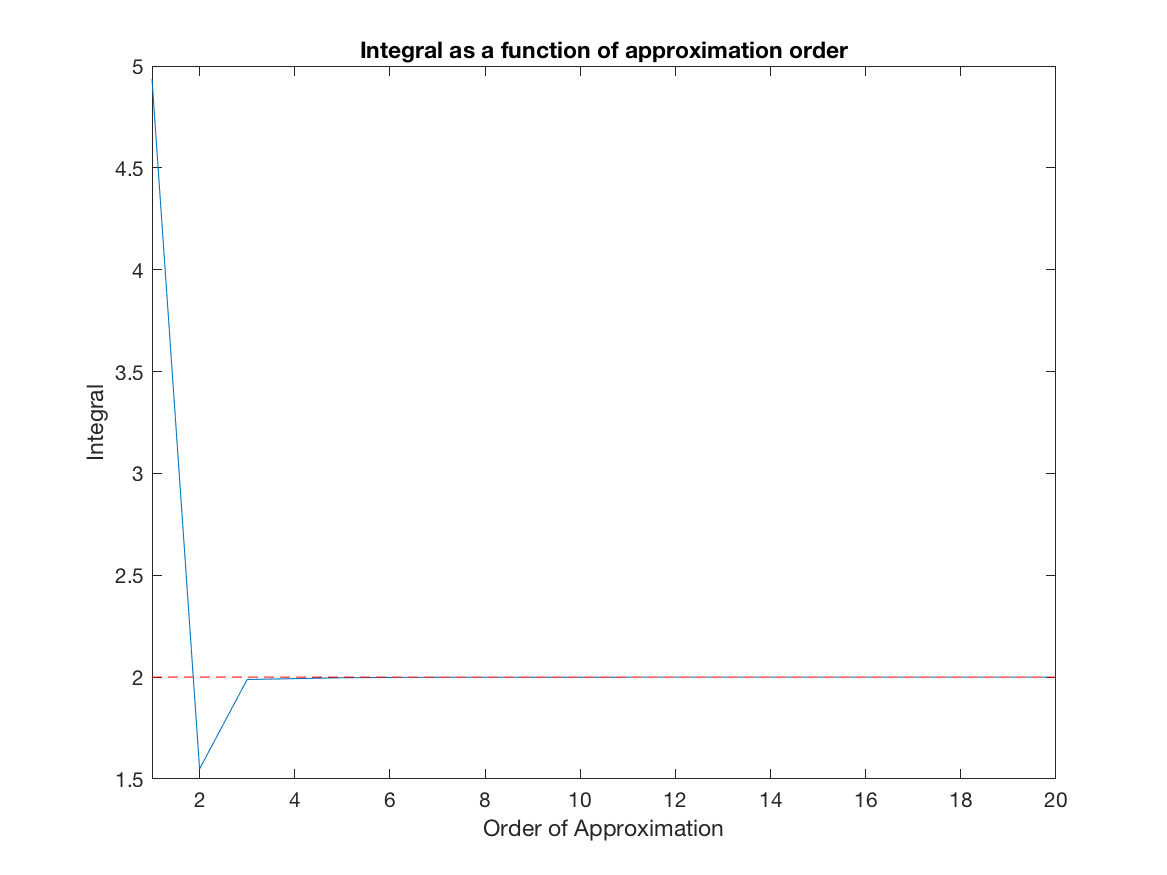
\includegraphics[scale=0.5]{Quad_1.png}
\end{figure}
Note: See Quadrature.m for details.
\end{frame}

\begin{frame}
\frametitle[alignment=center]{Example: $\sin(x)$}
\begin{figure}
\centering
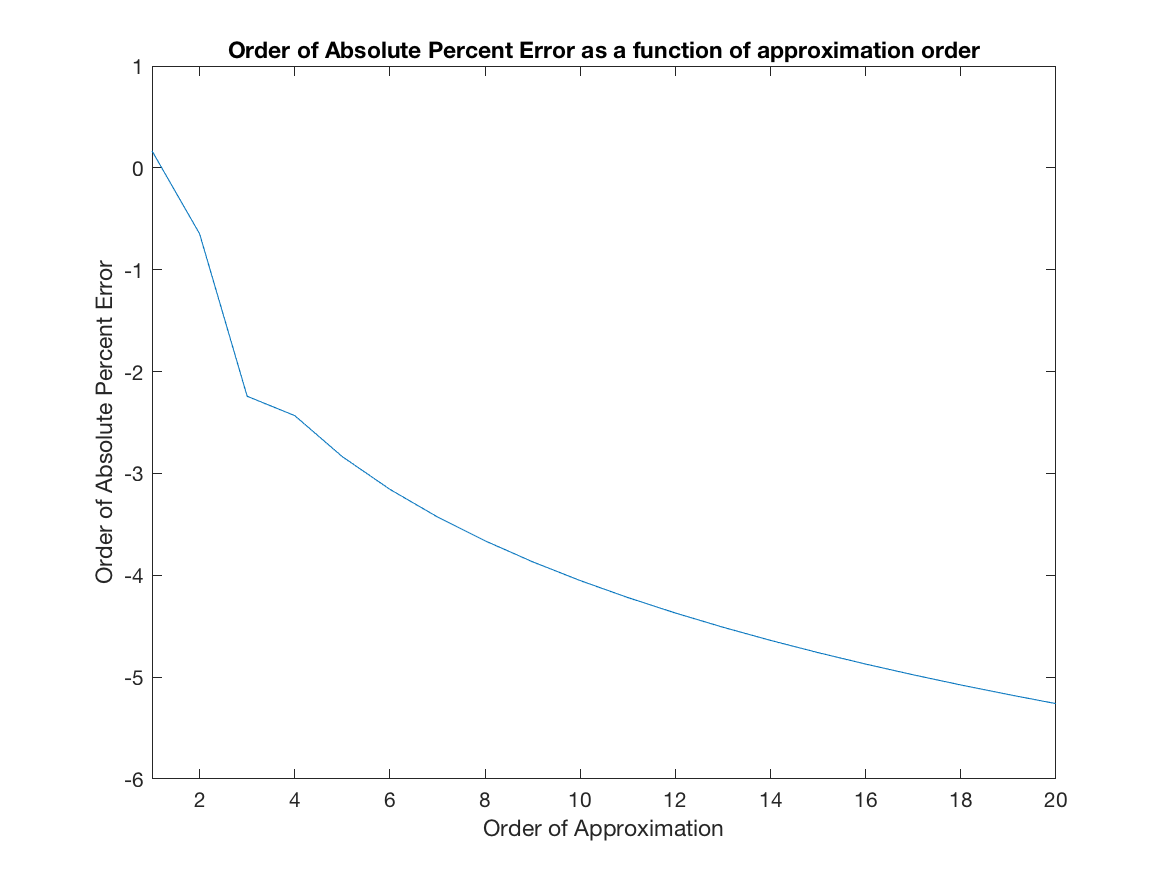
\includegraphics[scale=0.5]{Quad_2.png}
\end{figure}
Note: See Quadrature.m for details.
\end{frame}

\begin{frame}
\frametitle[alignment=center]{Matlab}
\begin{itemize}
\item There's a new guy in town
\bigskip
\item Don't exert thousands of (particularly valuable) man-hours picking the best polynomials and best points to maximize computational efficiency and running horse races
\bigskip
\item Nested sets of points to narrow things down is one option
\bigskip
\item Or, zoom in on trouble spots, make a more fine approximation there (Adaptive quadrature)
\bigskip
\item Adaptive sparse grid interpolation
\bigskip
\item Matlab: Sparse Grid Interpolation Toolbox by Andreas Klimke
\end{itemize}
\end{frame}

\begin{frame}
\frametitle[alignment=center]{Brumm \& Scheidegger (2015)}
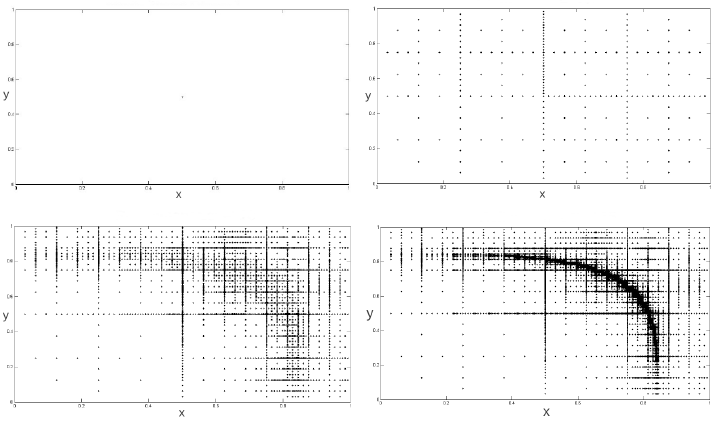
\includegraphics[scale=0.4]{Brumm_Scheidegger_2015_1.png}
\end{frame}

\begin{frame}
\frametitle[alignment=center]{Brumm \& Scheidegger (2015)}
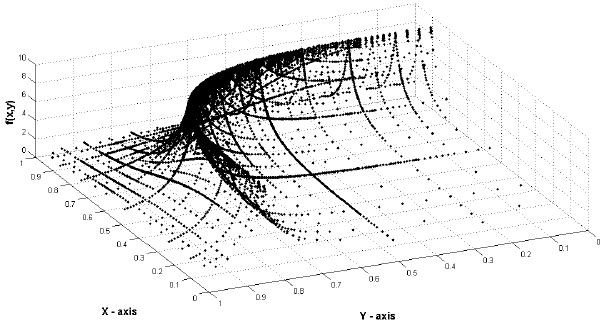
\includegraphics[scale=0.4]{Brumm_Scheidegger_2015_2.png}
\end{frame}

\begin{frame}
\frametitle[alignment=center]{Judd, Maliar, Maliar, and Valero}
\begin{itemize}
\item Taking every point in grid is inefficient
\bigskip
\item Good quick easy toolbox to interpolate and integrate functions on hypercubes
\bigskip 
\item Sparse grids can allow you to up your dimensions dramatically
\bigskip 
\item What does the grid look like?
\end{itemize}
\end{frame}

\begin{frame}
\frametitle[alignment=center]{Judd, Maliar, Maliar, and Valero}
\begin{figure}
\centering
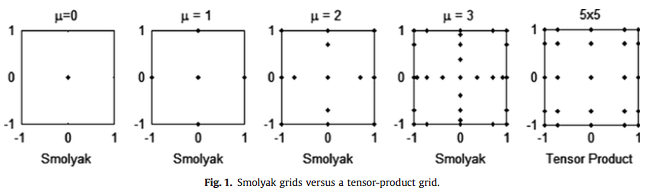
\includegraphics[scale=0.5]{Smolyak_1.png}
\end{figure}
\end{frame}

\begin{frame}
\frametitle[alignment=center]{Judd, Maliar, Maliar, and Valero}
\begin{figure}
\centering
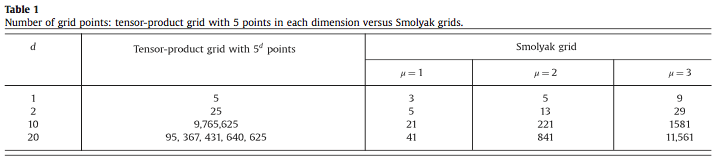
\includegraphics[scale=0.45]{Smolyak_2.png}
\end{figure}
\end{frame}

\begin{frame}
\frametitle[alignment=center]{Later in the Quarter: Monte Carlo Methods}
\begin{itemize}
\item Analytical integration isn't always possible
\bigskip
\item Numerical quadrature frequently focuses on and has good properties in a few dimensions
\bigskip
\item Monte Carlo integration has become popular
\bigskip
\item We'll talk about this a little later, but the idea is simple
\bigskip
\item ``Randomly$"^*$ walk around the space under the integral and sample points
\bigskip
\item Your ``sample" will be representative of the ``population" so you can add it up, average it, etc.
\bigskip
\item This can be hundreds of thousands of times less efficient, but it's also easy
\end{itemize}
\end{frame}



\end{document}